\section{Results from the Pilot Deployment}
\label{sec:pilot-study}

To evaluate the capabilities of the OPQ Sensor Network, 16 OPQ Boxes were deployed at the University of Hawaii Manoa campus over the course of three months in the Fall of 2019.  The University of Hawaii campus is an isolated microgrid connected to the Oahu powergrid only via a single 46kV feeder. The UH Campus also has commercial electrical meters (a mixture of GE PQMII and GE EPM 7000) deployed across various levels of the power delivery infrastructure. While the primary purpose of these meters is to monitor power consumption, they do include power quality monitoring capabilities. Data from these meters were used as ground truth for validation studies of the OPQ sensor network.

The University of Hawaii power grid is interesting in that it supplies a highly diverse infrastructure. Beyond traditional residential equipment such as computers and consumer grade electronics, the UH power grid powers scientific and laboratory equipment, machine shops, and server farms. All of these elements have varying requirements/tolerances for power quality anomalies as well as different levels of power quality “pollution”. Furthermore, some of the electricity consumers in the UH campus are entirely unique. For example, the free electron laser located in the Watanabe Hall is one of only ten in the world, and the impact/sensitivity of power quality on the instrument are completely unstudied.

The pilot study had the following major goals:

\begin{enumerate}

\item {\em Evaluation of sensor data accuracy and quality.} While we conducted extensive laboratory tests of the sensor network, the pilot study enabled us to evaluate the accuracy and utility of our hardware devices and power quality data collection procedures in a real-world setting. Does an OPQ sensor network measure power quality (and detect anomalies) as well or better than conventional building-level electrical meters?

\item {\em Evaluation of the triggering system.} The OPQ Makai triggering system provides a novel two-way communication between sensors and the cloud, resulting in a triggering system with unique capabilities.  Does the triggering system provide efficiencies not available from more conventional approaches? Does it provide data enabling analysis opportunities not available through more conventional approaches?

\item {\em Evaluation of the information architecture.} OPQ Mauka implements a tiered, hierarchical information architecture.  The pilot study enabled us to evaluate this information architecture.  Would this information architecture prove useful with real world data? Could actionable insights emerge from low-level sensor data?

\item {\em Evaluation of cloud data storage management.} OPQ Mauka manages data storage through a "time to live" (TTL) mechanism, which results in data being discarded if it is not found to be useful and thus "promoted" to a higher level of the information hierarchy within a defined period of time.  The pilot study enables us to evaluate this approach. Does this mechanism allow sensor network designers to determine upper bounds on storage requirements? Is information thrown away prematurely because it was not found to be useful within the time limits?

\end{enumerate}

Our pilot study is significant because much of the literature on power quality assessment relies on models, not actual installations \cite{anurangi_effects_2017,bayindir_effects_2016,farhoodnea_power_2012,shafiullah_experimental_2014}. In other cases, data was collected from only one location or for a very short time span \cite{kucuk_assessment_2013,viciana_openzmeter_2018}.

\subsection{Descriptive statistics}

The pilot study started on October 7, 2019 and ended on February 4, 2020. We deployed 16 OPQ Boxes across campus. As noted above, each OPQ Box collects 200 measurements per grid cycle, for a total of approximately 1B raw measurements per day per box.  Values for the maximum and minimum voltage, frequency, and THD, along with the presence or absence of transients, is sent once a second to the cloud by each box. Thus, each box sends approximately 86,400 measures per day to the cloud at a minimum. Over the course of the pilot study, a total of approximately 116M aggregate measures were sent by all of the OPQ Boxes.

Figure \ref{fig:statistics} provides two additional sets of summary statistics regarding the pilot study.  Figure (a) shows the number of anomalous events (i.e. where threshold values for frequency, voltage, THD, or transients were exceeded) along with the number of OPQ Boxes that experienced the power quality anomaly during that same time period. So, for example, 170,925 power quality anomalies were experienced by only one of the 16 OPQ boxes, and 463 anomalous power quality measurements were experienced by all 16 OPQ Boxes.

\begin{figure}[ht]
	\centering
	\begin{subfigure}{.5\textwidth}
        \begin{tabularx}{\textwidth}{XXXX|}
            \toprule
            \textbf{Events} & \textbf{Boxes} & \textbf{Events} & \textbf{Boxes} \\
            \midrule
            170,925 & 1 & 203 & 9 \\
            1,654 & 2 & 160 & 10 \\
            1,109 & 3 & 162 & 11 \\
            853 & 4 & 130 & 12 \\
            593 & 5 & 169 & 13 \\
            416 & 6 & 210 & 14 \\
            354 & 7 & 477 & 15 \\
            246 & 8 & 463 & 16 \\
             &  &  &  \\
            \bottomrule
        \end{tabularx}
	  \caption{Summary statistics: Events}
	\end{subfigure}%
	\begin{subfigure}{.5\textwidth}
	 \begin{tabularx}{\textwidth}{lX}
               \toprule
               \textbf{Incident} & \textbf{Total}  \\
               \midrule
               Frequency Swell & 291,235 \\
               Frequency Sag & 244,286  \\
               Excessive THD & 21,395 \\
               Voltage Sag & 620 \\
               ITIC (No Damage) & 93 \\
               SEMI F47 (Violation) & 24 \\
               Voltage Interruption & 16 \\
               Frequency Interruption & 14 \\
               Voltage Swell & 8 \\
               \bottomrule
           \end{tabularx}
   	  \caption{Summary statistics: Incidents}
	\end{subfigure}
	\caption{Summary statistics of (a) boxes involved in events and (b) incident type occurrences}
	\label{fig:statistics}
\end{figure}

\subsection{OPQ provides valid and reliable collection of power quality data}

The first goal of the pilot study was to assess how well an OPQ sensor network is able to collect basic power quality data. To do this, we compared data on voltage and frequency collected by OPQ Boxes with data on voltage and frequency collected by the existing UH power monitors.  The results are shown in Figure \ref{fig:opqbox-f-v-validation}.

\begin{figure}[ht]
	\centering
	\begin{subfigure}{.5\textwidth}
	  \centering
	  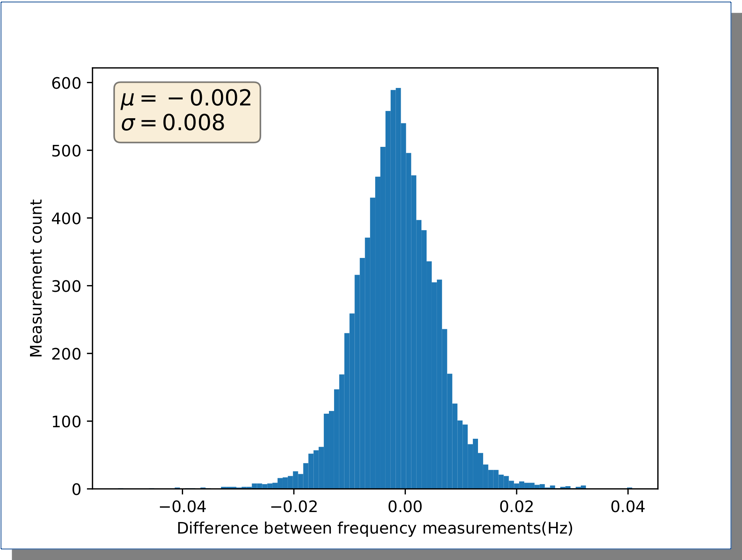
\includegraphics[width=0.9\linewidth]{images/pilot/opqbox-frequency-validation.png}
	  \caption{Frequency differences}
	  \label{fig:opqbox-validation-1}
	\end{subfigure}%
	\begin{subfigure}{.5\textwidth}
	  \centering
	  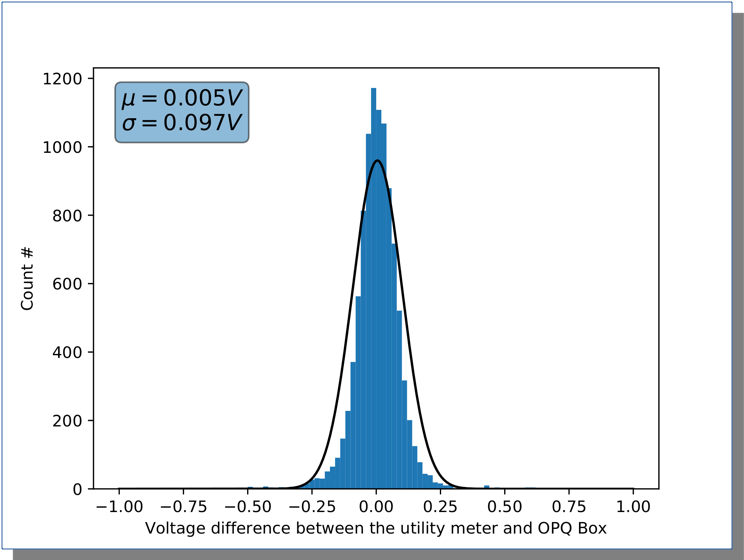
\includegraphics[width=0.9\linewidth]{images/pilot/opqbox-voltage-validation.png}
	  \caption{Voltage differences}
	  \label{fig:opqbox-validation-2}
	\end{subfigure}
	\caption{Validation of (a) Frequency and (b) Voltage}
	\label{fig:opqbox-f-v-validation}
\end{figure}

As the charts illustrate, there is very close correspondence between the building meters and the OPQ Boxes. For frequency differences, the value of $\sigma$ is 0.0079 Hz, and for voltage, $\sigma$ is 0.1703 V. (Note that typical thresholds for frequency and voltage PQ anomalies is 1 Hz and 6 V, so OPQ Box values appear accurate enough for their intended purpose.)

Validating THD and transient data, the other two basic power quality measures collected by OPQ Boxes, was more challenging.

Figure \ref{fig:opqbox-thd-validation} shows the results of comparing values of THD collected by OPQ Boxes and building meters.

\begin{figure}[ht]
  \centering
	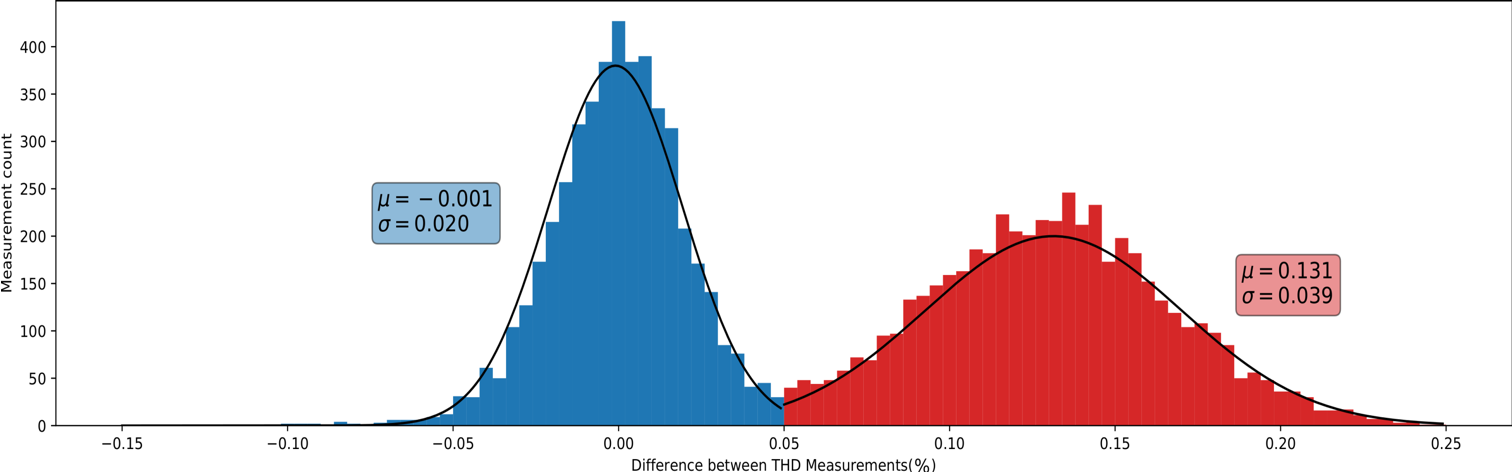
\includegraphics[width=0.8\linewidth]{images/pilot/opqbox-thd-validation.png}
	\caption{THD differences}
	\label{fig:opqbox-thd-validation}
\end{figure}

During the hours of 6pm and 6am, OPQBox and the building level meter displayed a high level of agreement as shown in the blue histogram in Figure \ref{fig:opqbox-thd-validaton}.
On the other hand, during the hours of 6pm and 6am, there was a static disparity of 0.13\% between the two meters as portrayed  in the red histogram.
This is likely attributed to the meter location in the power transmission hierarchy.
While the OPQ Box is plugged the $120V_{ac}$ line, the building meter is monitoring the $480V_{ac}$ three phase line.
An additional active conditioning system installed along side the transformer responsible for compensating for reactive power in the building is the likely culprit in the disparity.

Unfortunately, we unable to perform validation of transient data collection, because building meters did not provide us with access to that information. 
However, synthetic test performed in the lab against a calibration source, showed that OPQ Box is able to measure transient magnitude with $\sigma=0.125V$, significantly higher then the triggering threshold.
It should be noted that the internal transient metric provided by the OPQ Box is only used for event detection, while higher level analytics compute their own transient classification parameters.
As such, the transient detection capabilities of the OPQ Box are more then sufficient for its role in the OPQ ecosystem.

\subsection{OPQs triggering system provides advantages with respect to bandwidth and computation}

The pilot study provided an opportunity to collect data on the resources required by an OPQ sensor network with respect to cloud-level network resources and server-level computation overhead.

To assess network bandwidth utilization, we analyzed the data stream of frequency and voltage collected by OPQ Boxes, and the resulting network bandwidth utilized by the OPQ Makai triggering algorithm. Over the course of a typical day, OPQ Makai requested approximately 136 MB of data from the deployed OPQ Boxes.  We then calculated how much data would be sent by a power quality meter using more conventional triggering approach in which exceeding a threshold would automatically result in sending waveform data, and found that, under the same conditions, approximately 1025 MB would be sent to the cloud, or eight times the network bandwidth.

\begin{tcolorbox}[colback=blue!5!white,colframe=blue!75!black,title=SERGE]
Please review and improve the above paragraph.
\end{tcolorbox}

To assess computational cost, we again analyzed the data stream for a typical day...

\begin{tcolorbox}[colback=blue!5!white,colframe=blue!75!black,title=SERGE]
Please finish the above paragraph by describing in words the histogram in slide 38 of your thesis defense presentation, where you show that Napali uses much less computational resources.
\end{tcolorbox}

\subsection{OPQ enables subthreshold event detection based on temporal locality}
\label{sec:subthreshold-events}

One interesting capability enabled by two way communication between OPQ Boxes and their cloud-based services is what we term {\em subthreshold event detection based on temporal locality}.  In a nutshell, when one OPQ Box determines that a power quality measure has exceeded a threshold, one of the actions of the sensor network is to request high fidelity wave form data from neighboring boxes for the same temporal period, regardless of whether those boxes are reporting over-threshold data. In the event that any of those boxes actually do report over-threshold data, then the request ripples outward to the boxes neighboring that box, and so forth.

During the pilot study, we discovered several situations in which the OPQ sensor network was able to characterize power quality anomalies in the UH microgrid in a manner that the building level meters could not. For example...

\begin{tcolorbox}[colback=blue!5!white,colframe=blue!75!black,title=SERGE]
Please finish the above paragraph by describing one situation of subthreshold event detection and why it was cool.
\end{tcolorbox}

\subsection{The OPQ Information Architecture provides a means to produce actionable insights}

Figure \ref{fig:level-statistics} provides some descriptive statistics on the total number of entities created at each layer of the OPQ Information Architecture over the course of the pilot study. Note that the number of entities at a given layer at a given point in time is typically far less, due to the use of TTL to discard entities not promoted to higher layers.

\begin{figure}[ht]
  \centering
		 \begin{tabularx}{.4\textwidth}{lX}
       \toprule
       \textbf{Level} & \textbf{Total}  \\
       \midrule
       Phenomena & 10.4K \\
       Incidents & 415K \\
       Detections & 91.4K \\
       AML (Trends) & 1.94M \\
       AML (Measurements) & 116 M \\
       IML  & 100B \\
       \bottomrule
     \end{tabularx}
	\caption{Entities created at each level of the OPQ Information Architecture during the pilot study}
	\label{fig:level-statistics}
\end{figure}

Figure \ref{fig:level-statistics} shows that all layers of the hierarchy were actively used. In addition, the system was able to produce actionable insights by automatically detecting periodic phenomena for two boxes, and then predicting future occurrences of power quality anomalies with over a 50\% success rate (in other words, the current implementation of predictive phenomena leads to a significant false positive rate, predicting twice as many future power quality anomalies as actually occurred). Improving the predictive capabilities is a topic of future research.

\subsection{The OPQ Information Architecture provides predictable upper bounds on storage resources}

Figure \ref{fig:data-management-graph} shows a graph that illustrates storage requirements both with and without TTL-based data removal.  As the graph shows, over the course of the three month period, we estimate that cloud-level storage requirements would have reached approximately 2.5TB if all data was kept.  However, due to TTL, the amount of data held in the cloud at the conclusion of the case study was only 100 GB.

\begin{figure}[ht]
  \centering
	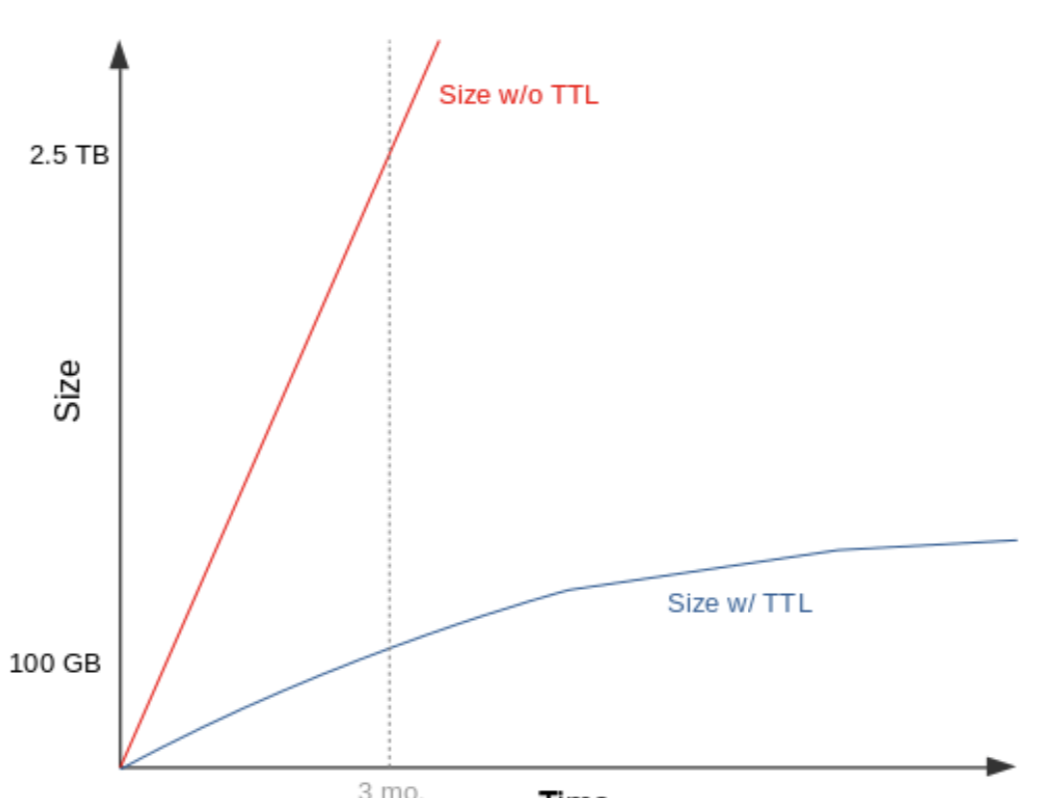
\includegraphics[width=0.4\linewidth]{images/pilot/data-management-graph.png}
	\caption{Storage requirements with and without TTL}
	\label{fig:data-management-graph}
\end{figure}

It is difficult to compute a strict upper bound on storage requirements for an OPQ network, because the amount of storage does depend on the number of power quality anomalies experienced by the grid. That said, we did notice that storage requirements were rising much more slowly at the end of the pilot when utilizing TTL as compared to not utilizing TTL.

The largest contribution to data storage is the raw power data. In a system without TTL, raw data storage rapidly grows. The bounds on raw storage can be calculated by taking into account the sampling rate and sample size for active OPQ Boxes as described in Equation ~\ref{eq:RawDataBytes}.

\begin{equation}
    RawDataBytes = NumBoxes * TimeSeconds * SampleRate * SampleSize
    \label{eq:RawDataBytes}
\end{equation}

Given that OPQ Boxes were configured to sample at 12 kHz at 2 bytes per sample during the deployment, we can calculate the bounds on raw storage for 16 OPQ Boxes over 3 months without TTL as 3.1 TiB. Figure~\ref{fig:data-management-graph} shows slightly less data as the number of OPQ Boxes was not constant during the pilot study (Figure~\ref{fig:active-opq-boxes}). By implementing TTL, significant data savings are made by discarding of IML data that is mostly noise.

\begin{figure}[ht]
    \centering
    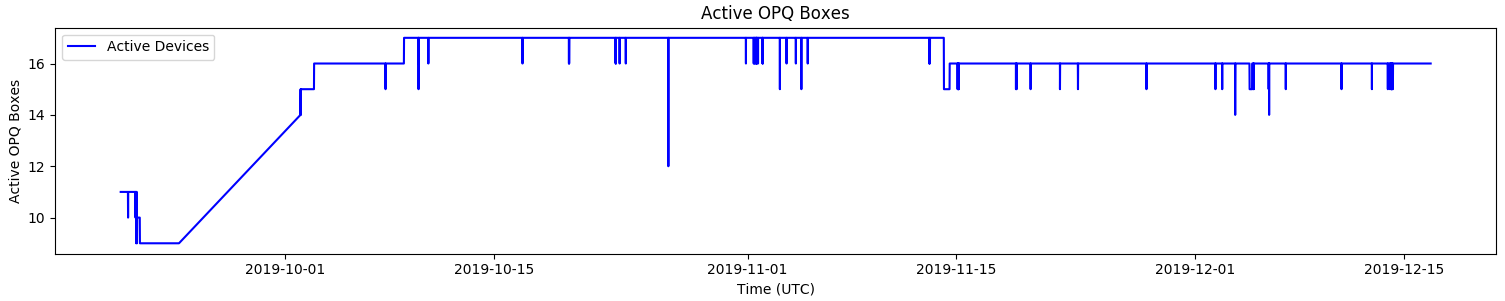
\includegraphics[width=0.75\linewidth]{images/pilot/active-opq-boxes.png}
    \caption{Active OPQ Boxes vs. Time}
    \label{fig:active-opq-boxes}
\end{figure}

Given a network of 16 OPQ Boxes over the pilot deployment period with TTL, the combined data storage from all levels reached an asymptotic limit of near 100 GB. The layout of data storage is provided per data storage level in Figure~\ref{fig:opq-data-storage}. The high rate of detections made by OPQ utilize most of the space. The reason for this is that Events store associated IML data along with each detection for high-fidelity analysis. It's also possible to observe how the AML and IML levels level off asymptomatically over time. This is a result of TTL discarding not useful data.

\begin{figure}[ht]
    \centering
    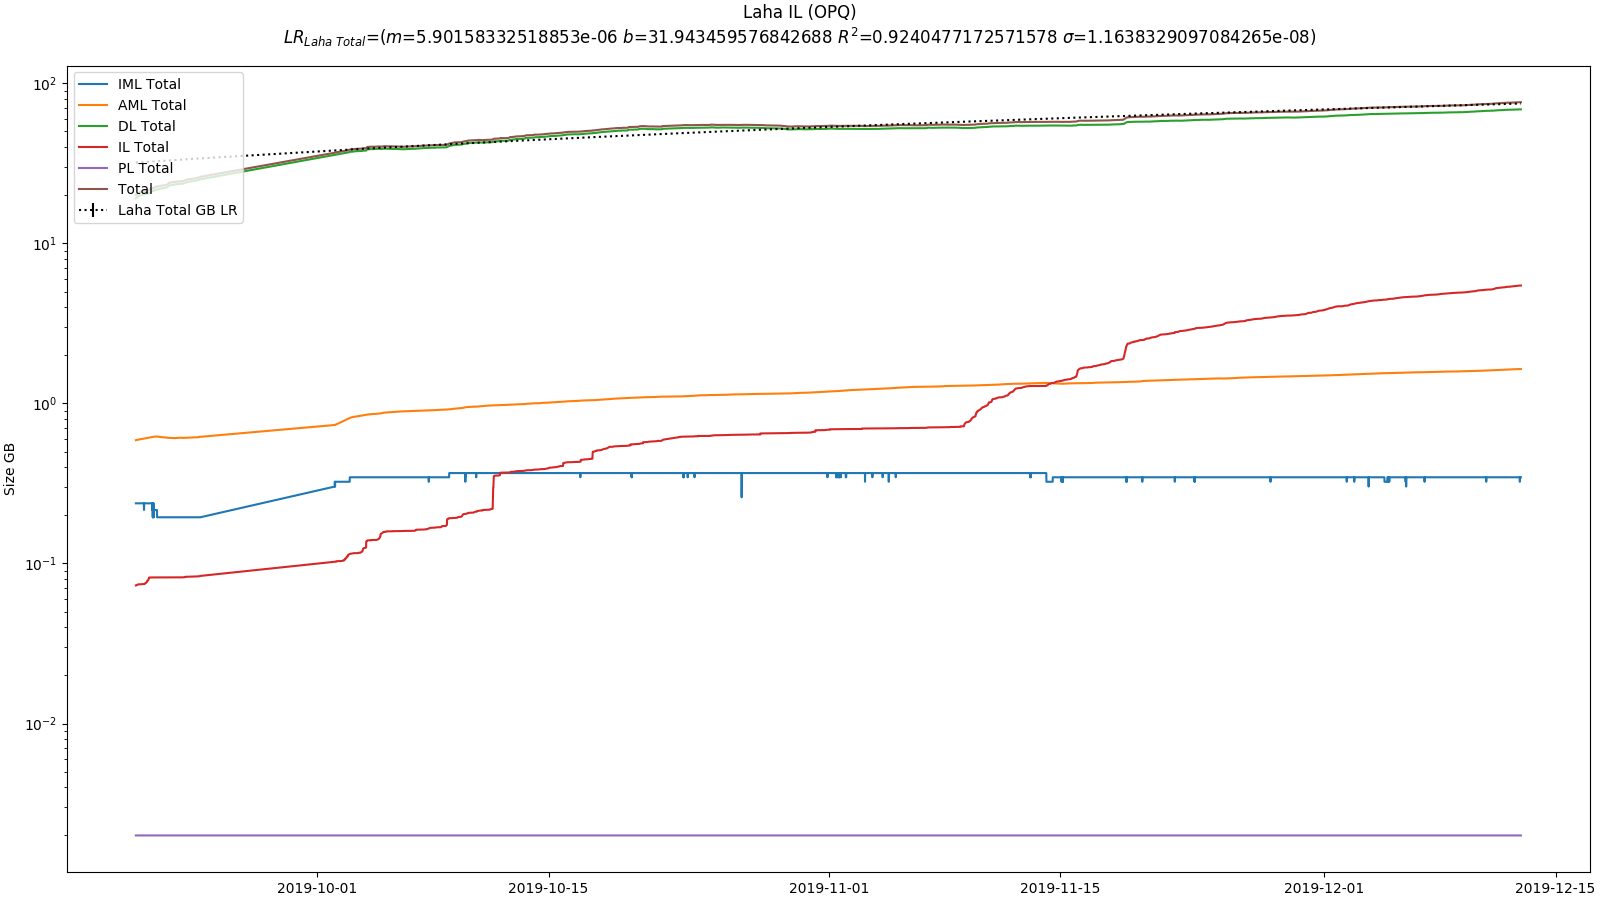
\includegraphics[width=0.75\linewidth]{images/pilot/laha-levels-storage.png}
    \caption{Combined OPQ Data Storage}
    \label{fig:opq-data-storage}
\end{figure}

\subsection{OPQ provides useful adaptive optimization capabilities}
\label{sec:adaptive-optimization}

The top layer of OPQ's information architecture supports adaptive optimization: the ability to analyze previously collected data and use it to change the settings associated with data collection from OPQ Boxes.

Two areas where adaptive optimizations were utilized are identifying periodic phenomena and predictions of future phenomena. Periodic phenomena are PQ related signals that occur at regular intervals. One example of periodic phenomena is a cyclic voltage sag that was observed at one of our sensors with a period of about 34 minutes during our pilot study (Figure~\ref{fig:periodic-voltage-sags}). This periodic phenomena not only provided a classification of an interesting pattern, but also helped optimize the OPQ system for capture of future phenomena. Several system wide optimizations are utilized.

\begin{figure}[H]
    \centering
    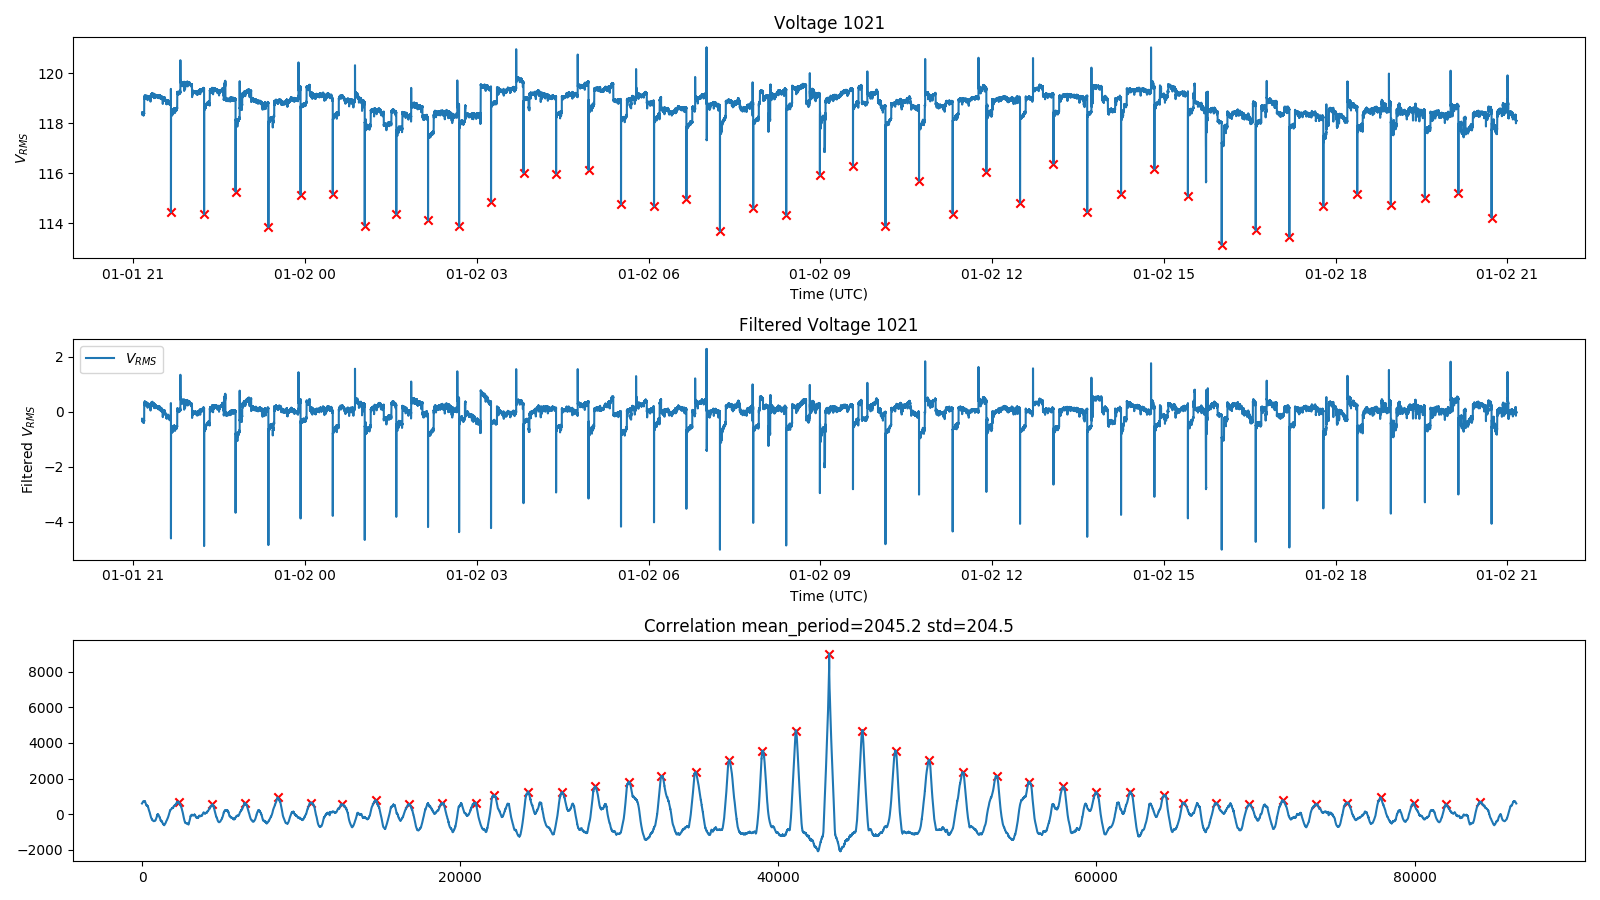
\includegraphics[width=0.75\linewidth]{images/pilot/periodic-voltage-sags.png}
    \caption{Detection of Periodic Voltage Sags}
    \label{fig:periodic-voltage-sags}
\end{figure}

First, classified periodic phenomena are used to generate future phenomena. Future phenomena are a prediction of future signals of interest. When a prediction is made, the system will automatically increase sampling fidelity for the predicted sensor during the time window of the prediction. In particular, the measurement rate is increased from 1 measurement per second to 6 measurements per second providing higher fidelity data. Detection thresholds are also decreased, making it more likely that the predicted signal will be observed even if it is of low magnitude.

As an example, Figure~\ref{fig:future-phenomena} shows the percentage of correctly predicted future phenomena as a function of time. The self-optimizing nature of the system allows the system to make more accurate predictions due to acting on more accurate periodic phenomena.

\begin{figure}[H]
    \centering
    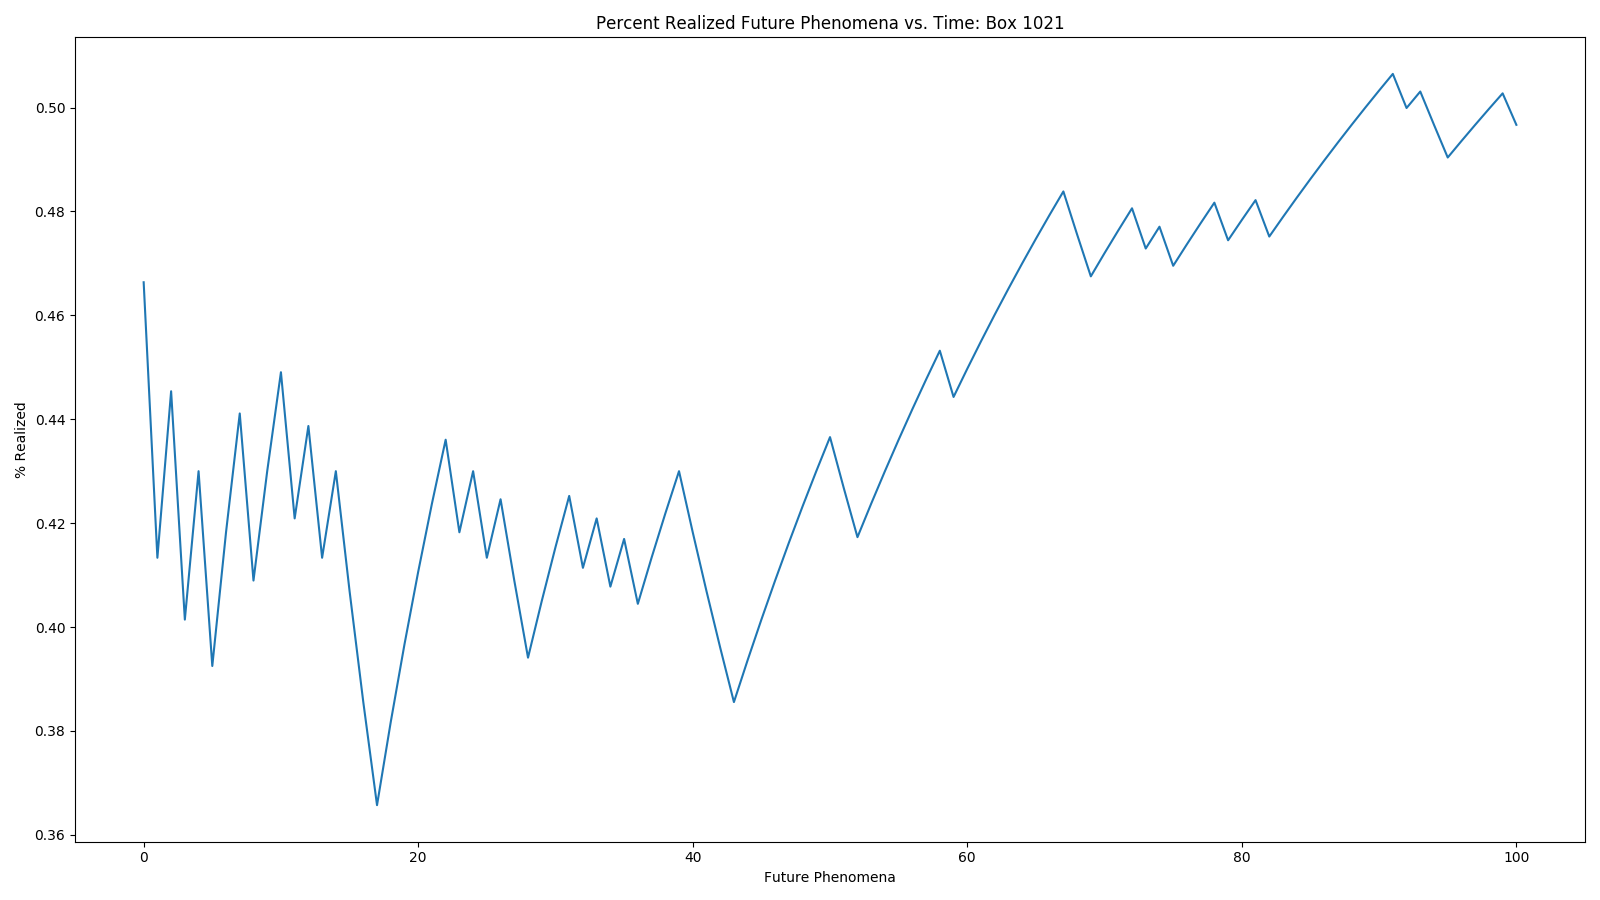
\includegraphics[width=0.60\linewidth]{images/pilot/realized-future-phenomena.png}
    \caption{Future Phenomena Prediction Accuracy Over Time}
    \label{fig:future-phenomena}
\end{figure}

Second, the increase in detection sensitivity makes it more likely that sub-threshold signals of interest will be classified. As example, the increased detection sensitivity allowed us to observe and classify a periodic voltage sag that would not have been detected by our normal classifier due to the small magnitude of the sag. The sub-threshold detection is shown in Figure~\ref{fig:sub-threshold-detection}.

\begin{figure}[H]
    \centering
    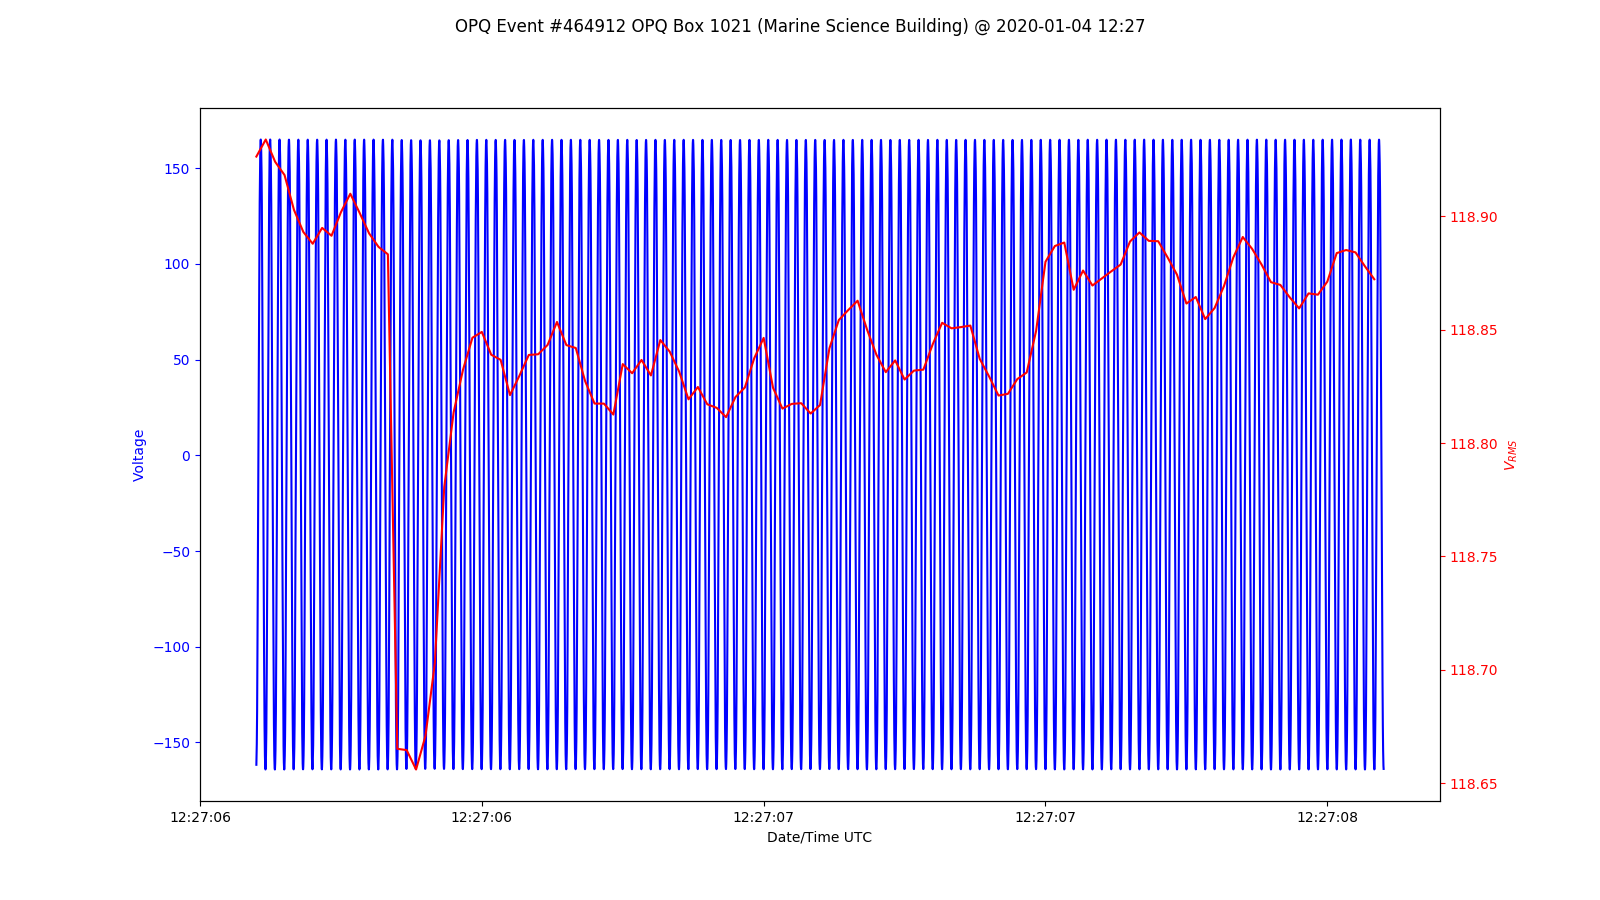
\includegraphics[width=0.85\linewidth]{images/pilot/subthreshold-signal.png}
    \caption{Sub-threshold Detection}
    \label{fig:sub-threshold-detection}
\end{figure}

This creates a positive feedback loop whereas periodic phenomena become more accurate, future phenomena become more accurate. As future phenomena become more accurate, periodic phenomena become more accurate.

\begin{tcolorbox}[title=ANTHONY AND SERGE]
Any other pilot study results that I've forgotten to include?
\end{tcolorbox}





